Using our newly constructed difference based extrapolation framework, we can now do the same analysis on our three nuclei \n{2}{H}, \n{3}{H} and \n{4}{He} using the same interaction as used earlier. Even though the difference based framework uses differences to compute a difference prediction internally, the final evaluation will still base off the same absolute energy differences and result in an absolute energy prediction. This means that we can apply our different evaluation modifications from \autoref{chap:extended} and discuss the influences of them on the difference based evaluation. Furthermore, using the same nuclei allows us to compare the difference based extrapolation and the absolute value extrapolation.

The results of our difference based extrapolation is shown in \autoref{fig:eval_diff}. The final extrapolated values and their uncertainty are shown in \autoref{tab:eval_diff} as well for each $N_\mathrm{max}$ and each SRG flow parameter.

% Generell: Predictions VIEL genauer, besonders bei hohem Nmax
% Generell: Trainingsmodes machen nicht mehr viel aus
% Kein unterbinden mehr -> "monoton steigende predictions" sind nicht mehr da
% He4 0.04 vs 0.08: Effekt von sehr unterschiedlichen sequenzen viel größer als bei abs (abs besser)
% 0.08: SRG hat viel mehr auswirkung als bei abs und bei 0.04
% H2: 0.08 schlechter als 0.04

\begin{table}[H]
  \caption{Extrapolation results in \si[]{\mega\electronvolt} of the difference based framework for the nuclei \n{2}{H} \textbf{(a)}, \n{3}{H} \textbf{(b)} and \n{4}{He} \textbf{(c)}. For each interaction characterized by the flow parameter $\eta = \srg{0.04}, \srg{0.08}$, the final extrapolation results for the given $N_\mathrm{max}$ value is shown. Here, \textbf{(1)} is our basic extrapolation without further modifications of the training step, \textbf{(2)} is the $N_\mathrm{max}$-limitation training mode, \textbf{(3)} is the SRG-filter training mode. }
  \label{tab:eval_diff}
  \centering
  \begin{subtable}{\textwidth}
    \caption{}
    \centering
    \begin{tabular}{
        r|
        S[table-format=-2.3(3)]
        S[table-format=-2.3(3)]
        S[table-format=-2.3(3)]
        S[table-format=-2.3(3)]
        S[table-format=-2.3(3)]
        S[table-format=-2.3(3)]
      }
      \toprule
      $\eta$                           &
      \multicolumn{3}{c}{$\srg{0.04}$} &
      \multicolumn{3}{c}{$\srg{0.08}$}   \\
      \midrule
      $N_\mathrm{max}$                 &
      {8}                              &
      {10}                             &
      {12}                             &
      {8}                              &
      {10}                             &
      {12}                               \\
      \midrule
      (1)                              &
      -2.066 \pm 0.065                 &
      -2.144 \pm 0.025                 &
      -2.129 \pm 0.022                 &
      -2.054 \pm 0.069                 &
      -2.113 \pm 0.028                 &
      -2.126 \pm 0.023                   \\
      (2)                              &
      -2.080 \pm 0.055                 &
      -2.146 \pm 0.023                 &
      -2.127 \pm 0.020                 &
      -2.064 \pm 0.056                 &
      -2.110 \pm 0.026                 &
      -2.124 \pm 0.022                   \\
      (3)                              &
      -2.068 \pm 0.055                 &
      -2.153 \pm 0.038                 &
      -2.149 \pm 0.034                 &
      -2.062 \pm 0.041                 &
      -2.124 \pm 0.032                 &
      -2.158 \pm 0.036                   \\
      \bottomrule
    \end{tabular}
  \end{subtable}
  \par\bigskip
  \begin{subtable}{\textwidth}
    \caption{}
    \centering
    \begin{tabular}{
        r|
        S[table-format=-2.3(3)]
        S[table-format=-2.3(3)]
        S[table-format=-2.3(3)]
        S[table-format=-2.3(3)]
        S[table-format=-2.3(3)]
        S[table-format=-2.3(3)]
      }
      \toprule
      $\eta$                           &
      \multicolumn{3}{c}{$\srg{0.04}$} &
      \multicolumn{3}{c}{$\srg{0.08}$}   \\
      \midrule
      $N_\mathrm{max}$                 &
      {8}                              &
      {10}                             &
      {12}                             &
      {8}                              &
      {10}                             &
      {12}                               \\
      \midrule
      (1)                              &
      -8.453 \pm 0.099                 &
      -8.528 \pm 0.044                 &
      -8.470 \pm 0.026                 &
      -8.410 \pm 0.090                 &
      -8.465 \pm 0.035                 &
      -8.460 \pm 0.025                   \\
      (2)                              &
      -8.461 \pm 0.082                 &
      -8.526 \pm 0.036                 &
      -8.468 \pm 0.025                 &
      -8.422 \pm 0.074                 &
      -8.464 \pm 0.031                 &
      -8.457 \pm 0.023                   \\
      (3)                              &
      -8.390 \pm 0.064                 &
      -8.493 \pm 0.028                 &
      -8.466 \pm 0.026                 &
      -8.408 \pm 0.045                 &
      -8.460 \pm 0.026                 &
      -8.466 \pm 0.025                   \\
      \bottomrule
    \end{tabular}
  \end{subtable}
  \par\bigskip
  \begin{subtable}{\textwidth}
    \caption{}
    \centering
    \begin{tabular}{
        r|
        S[table-format=-2.3(3)]
        S[table-format=-2.3(3)]
        S[table-format=-2.3(3)]
        S[table-format=-2.3(3)]
        S[table-format=-2.3(3)]
        S[table-format=-2.3(3)]
      }
      \toprule
      $\eta$                           &
      \multicolumn{3}{c}{$\srg{0.04}$} &
      \multicolumn{3}{c}{$\srg{0.08}$}   \\
      \midrule
      $N_\mathrm{max}$                 &
      {8}                              &
      {10}                             &
      {12}                             &
      {8}                              &
      {10}                             &
      {12}                               \\
      \midrule
      (1)                              &
      -28.502 \pm 0.397                &
      -28.497 \pm 0.212                &
      -28.405 \pm 0.095                &
      -28.520 \pm 0.175                &
      -28.535 \pm 0.064                &
      -28.529 \pm 0.025                  \\
      (2)                              &
      -28.399 \pm 0.319                &
      -28.454 \pm 0.177                &
      -28.391 \pm 0.080                &
      -28.522 \pm 0.143                &
      -28.537 \pm 0.052                &
      -28.530 \pm 0.021                  \\
      (3)                              &
      -28.377 \pm 0.294                &
      -28.408 \pm 0.139                &
      -28.353 \pm 0.054                &
      -28.507 \pm 0.065                &
      -28.521 \pm 0.026                &
      -28.527 \pm 0.012                  \\
      \bottomrule
    \end{tabular}
  \end{subtable}
\end{table}

a
\begin{figure}[H]
  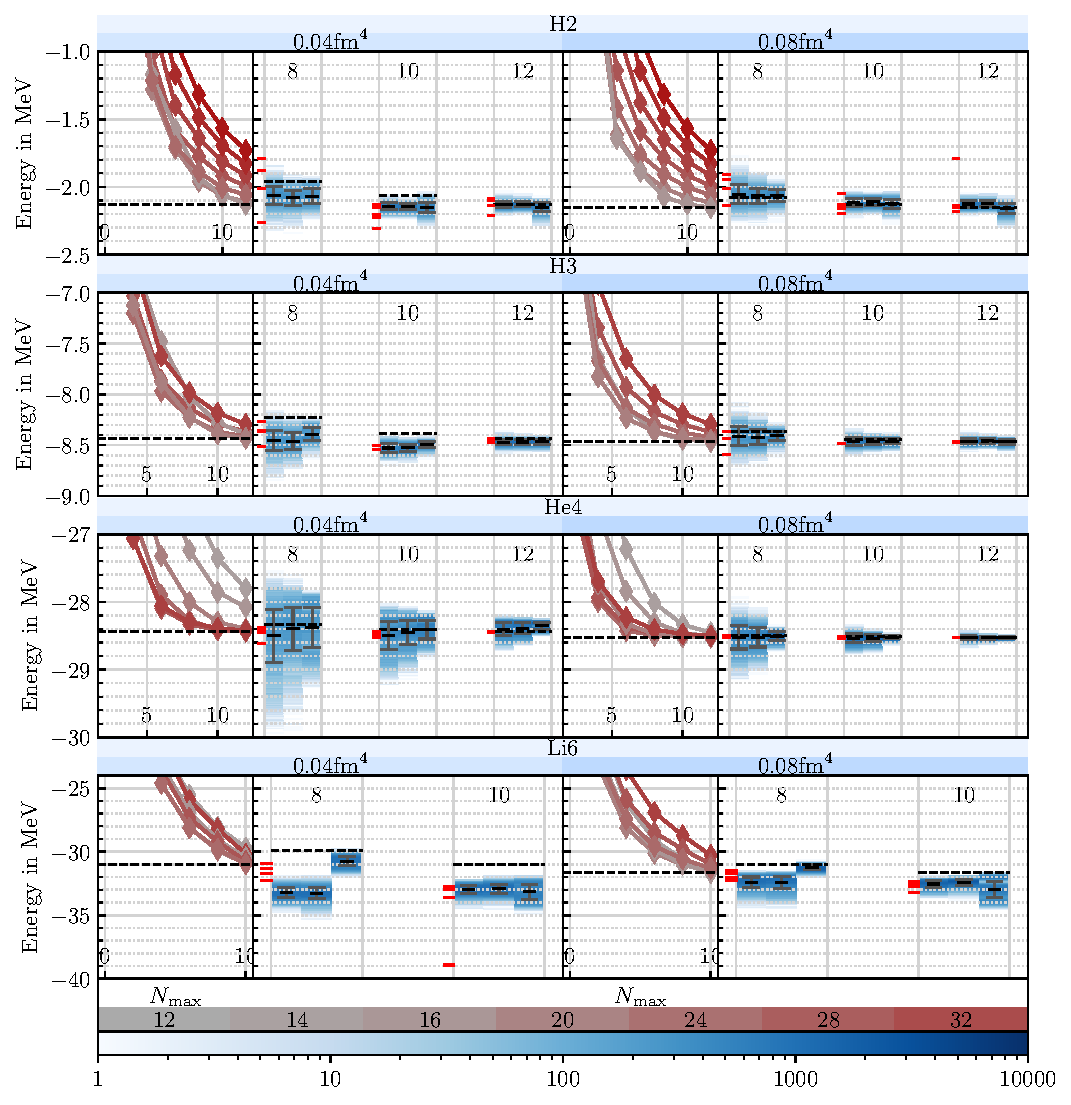
\includegraphics[width=\textwidth]{media/diff_evaluation.pdf}
  \caption{a}
  \label{fig:eval_diff}
\end{figure}

